% ~ 12 pages
\chapter{Identification of Hadronically Decaying $\tau$-Leptons (BDT)}
\label{sec:bdt}

\section{Features of Hadronically Decaying Tau Leptons}
\label{sec:features_tau_decay}

Features of hadronically decaying $\tau$-leptons vs. Quark/Gluon initiated jets:
\begin{itemize}
\item Low multiplicity (QCD jets usually have a lot of tracks)
\item Isolated tracks and narrow showers
\item Measurable decay length with proper lifetime of
  $\tau = \SI{290.3 +- 0.5}{\femto\second}$ \cite{pdg} and following from that
  $c \tau = \SI{87.0 +- 0.2}{\micro\metre}$ with $\beta \gamma = 10$ which
  corresponds to a roughly \SI{18}{\giga\electronvolt} tau the mean decay length
  is of the order of a millimetre and allows secondary vertex reconstruction or
  employing the impact parameter for 1-prong taus (sub-millimetre resolution).
\item Invariant mass bounds for decay products
\end{itemize}


\section{Event Simulation, Reweighting and Preselection}
\label{sec:bdt_eventsim}

\todo{Signal}
For training and performance evaluation simulated data is used. For tau
performance trainings and tunings a sample created by the process
$\gamma^* \rightarrow \tau \tau \, \text{(hadr.)}$ is used, where at
generator-level leptonic decays of the tau is disabled. Moreover interference
with and on-/ off-shell production of the $\mathrm{Z}^0$ boson is disabled. The
reason for not using a sample employing the Drell--Yan process including
interference and on- / off-shell production of the $\mathrm{Z}^0$ boson is that
the tau polarisation changes for di-tau invariant masses close to the
$\mathrm{Z}$-mass whereas unpolarised taus are desired. Moreover the di-tau mass
spectrum is smooth and decreasing without increased statistics close to the
$\mathrm{Z}$ mass which is not needed for performance studies.

\todo{Background} The background for the identification studies is given by
dijet samples up to \SI{1800}{\giga\electronvolt} (JZ1W - JZ6W). \todo{Finish
  this}

Basic tau selection
\begin{itemize}
\item $p_\text{T} > \SI{20}{\giga\electronvolt}$ (sufficient for most analyses)
\item Exclude calorimeter transition region $1.37 < |\eta| < 1.52$
\item Require tracker acceptance region $|\eta| < 2.5$
\item One or three reconstructed tracks
\item Truth-matching for signal events ($p_\text{T}$, $\eta$ and
  $N_\text{track}$ selection also at truth-level)
\end{itemize}

\todo{Sample sizes after basic selection}

\todo{Reweighting}

A full summary of the datasets is given in appendix \todo{Reference}.

\section{Description of the Tau-Identification Procedure}
\label{sec:bdt_tauid}

\subsection{Features (Predictors, Dependent Variables, Input Variables)}
\label{sec:bdt_features}

Input variables
\begin{itemize}
\item Central energy fraction $f_\text{cent}$ (1P, 3P)
\item etOverPtLeadTrk $f_\text{leadtrack}^{-1}$ (1P, 3P)
\item innerTrkAvgDist $R_\text{track}^{0.2}$ (1P, 3P)
\item absipSigLeadTrk $\left| S_\text{leadtrack} \right|$ (1P)
\item SumPtTrkFrac $f_\text{iso}^\text{track}$ (1P)
\item ChPiEMEOverCaloEME $f_\text{EM}^\text{track-HAD}$ (1P, 3P)
\item EMPOverTrkSysP $f_\text{track}^\text{EM}$ (1P, 3P)
\item ptRatioEflowApprox $p_\text{T}^\text{EM+track} / p_\text{T}$ (1P, 3P)
\item mEflowApprox $m_\text{EM+track}$ (1P, 3P)
\item dRmax $\Delta R_\text{max}$ (3P)
\item trFlightPathSig $S_\text{T}^\text{flight}$ (3P)
\item massTrkSys $m_\text{track}$ (3P)
\end{itemize}

Setup
\begin{itemize}
\item NTrees: 100
\item MaxDepth: 8
\item AdaBoostBeta: 0.2
\item MinNodeSize: 0.1
\item nCuts: 200
\item UseYesNoLeaf: False
\item PruneMethod: NoPruning
\end{itemize}
Previous setup (incl. explanation \& plots of input variables)

Transformations?

\section{Hyperparameter Optimisation}
\label{sec:bdt_hyperparam}

TMVA \cite{tmva}.

Quickly describe previous setup.

Before proceeding to feature selection a reliable hyperparameter setup has to be
found.

Pick the best-performing BDT \& a good compromise between 'overtraining' and
performance.

Optimised for tight efficiency w/o subsampling:
\begin{itemize}
\item \textbf{Best performance 1P:} MaxDepth: 16, MinNodeSize: 0.01, NTrees:
  400, Shrinkage: 0.05, ratio: 0.997 \textrightarrow alg 244
\item \textbf{Compromise 1P:} MaxDepth: 8, MinNodeSize: 0.1, NTrees: 400,
  Shrinkage: 0.1, sumsampling: 50\%, ratio: 0.977 \textrightarrow alg 321
\item \textbf{Best performance 3P:} MaxDepth: 16, MinNodeSize: 0.01, NTrees:
  400, Shrinkage: 0.4, ratio: 0.998 \textrightarrow 259
\item \textbf{Compromise 3P:} MaxDepth: 6, MinNodeSize: 0.1, NTrees: 800,
  Shrinkage: 0.4, ratio: 0.964 \textrightarrow alg 327
\end{itemize}

\subsection{Boosting Algorithm}
\label{sec:bdt_boosting}

AdaBoost \textrightarrow GradBoost

\subsection{Exhaustive Grid Search}
\label{sec:bdt_grid_search}

\begin{align*}
  N_\mathrm{Trees} &\in \{25, 50, 100, 200, 400, 800\} &
  d_\mathrm{Tree} &\in \{4, 6, 8, 12, 16\} \\
  \eta &\in \{0.05, 0.1, 0.2, 0.4\} &
                                      f_\mathrm{Node}^\mathrm{min.} &\in \{\SI{0.01}{\percent}, \SI{0.1}{\percent},\SI{1.0}{\percent}\} \\
  f_\text{bag} &\in \{\text{None}, \SI{50}{\percent} \}
\end{align*}
Total of $6 \times 5 \times 4 \times 3 \times 2 = 720$

TMVA Grid Search
XGBoost (?)
Comparison with previous setup

\begin{figure}[ht]
  \begin{subfigure}[t]{0.48\textwidth}
    \centering
    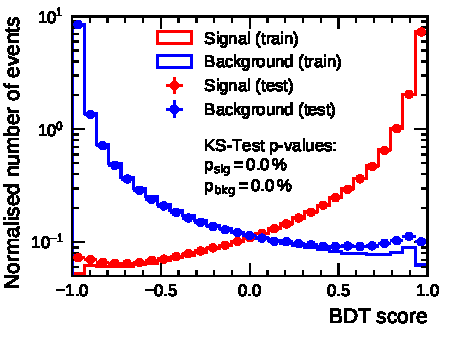
\includegraphics{./figures/bdt_perf/scores/grid_1p0304.pdf}
    \subcaption{Overtrained example:
      \mbox{$N_\text{Trees} = 800$},
      \mbox{$d_\text{Tree} = 16$},
      \mbox{$\nu = 0.05$, $f_\text{min.}^\text{Node} = \SI{0.01}{\percent}$},
      no bagging
    }
  \end{subfigure}\hfill
  \begin{subfigure}[t]{0.48\textwidth}
    \centering
    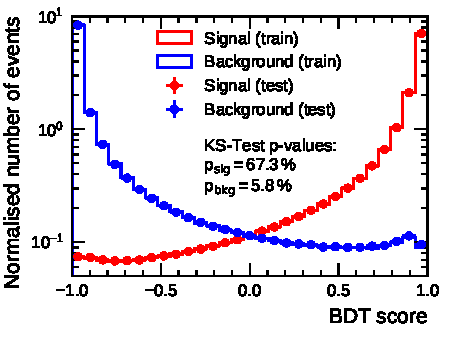
\includegraphics{./figures/bdt_perf/scores/grid_1p_subsampling0269.pdf}
    \subcaption{Good training:
      \mbox{$N_\text{Trees} = 400$},
      \mbox{$d_\text{Tree} = 8$},
      \mbox{$\nu = 0.1$, $f_\text{min}^\text{Node} = \SI{0.1}{\percent}$},
      \mbox{$f_\text{bag} = \SI{50}{\percent}$}
    }
  \end{subfigure}
  \caption{'Overtraining' visible on the edges of the BDT score distribution}
  \label{fig:bdt_1p_scores}
\end{figure}


\subsection{Working Points}
\label{sec:bdt_working_points}

Working points (Gammatautau -- Ztautau)

Signal efficiencies 1P (3P):
\begin{itemize}
\item Very Loose: 95\% (95\%)
\item Loose: 85\% (75\%)
\item Medium: 75\% (60\%)
\item Tight: 60\% (45\%)
\end{itemize}

\section{Feature Selection}
\label{sec:bdt_feature_selection}

\subsection{Variable Importance}
\label{sec:bdt_var_importance}

Variable correlations, importance (dropped variables) \& dependence with
$p_\mathrm{T}$ (2D Hist - including pt), Variable Transformations (instead
of cutting out outliers), Partial Dependence, Including $p_\mathrm{T}$

\section{Identification Performance on Simulated Data}
\label{sec:bdt_perf}

\subsection{Performance in Simulation}
\label{sec:bdt_perf_sim}

Impact on (reconstructed) decay modes (?)

\subsubsection{Performance on Quark- / Gluon-initiated Jets}
\label{sec:bdt_perf_quark_gluon}

Impact of Quark / Gluon initiated jets on Tau-ID (i.e. performance of ID
on Quark / Gluon jets)

\subsection{Performance on Data}
\label{sec:bdt_perf_data}

Performance on TAUP4 (?)

% -------------------------------------------------------------------------- %
\begin{itemize}
\item Description \& Plots of the input variables
  \begin{itemize}
  \item How does etOverPtLeadTrk differ from EMPOverTrkSysP for 1-prong taus?
  \end{itemize}

\item Preselection
  \begin{itemize}
  \item $p_\mathrm{T} > \SI{20}{\GeV}$ (reconstructed \& truth)
  \item $| \eta | < 2.5$ (reconstructed \& truth)
  \item $| \eta | \notin \left[ 1.37, 1.52 \right]$ (reconstructed \& truth)
  \item truth-matched taus
  \end{itemize}

\item Train baseline for comparison (with default outlier removal)
  \begin{itemize}
  \item NTrees 100 (explain)
  \item MinNodeSize 0.1 (explain)
  \item BoostType AdaBoost (explain)
  \item SeparationType GiniIndex (explain)
  \item PruneMethod NoPruning
  \item UseYesNoLeaf False (explain)
  \item AdaBoostBeta 0.2 (explain)
  \item DoBoostMonitor True
  \item nCuts 200 (explain)
  \item MaxDepth 8 (explain)
  \end{itemize}

\item Switch from AdaBoost to GradBoost (Explain why we don't do a full
  optimization of the AdaBoost vs GradBoost setup)

\item Variable transformations (log, clamp, uniformization)
  \begin{align}
    &\text{SumPtTrkFrac:} &\log(x + 10^{-4}) \\
    &\text{absipSigLeadTrk:} &\min(x, 30) \\
    &\text{mEflowApprox:} &\log(x) \\
    &\text{centFrac:} &\min(x, 1) \\
    &\text{innerTrkAvgDist:} &- \\
    &\text{ptRatioEflowApprox:} &\min(x, 4) \\
    &\text{EMPOverTrkSysP:} &\log(\max(10^{-3}, x)) \\
    &\text{etOverPtLeadTrk:} &\log(\max(0.1, x)) \\
    &\text{ChPiEMEOverCaloEME:} &\max(-4, \min(x, 5)) \\
    &\text{trFlightPathSig:} &\log(\max(0.01, x)) \\
    &\text{massTrkSys:} &\log(x) \\
    &\text{dRmax:} &-
  \end{align}

\item BDT optimization for R21 (Total 480 BDTs) -- If enough time try 50\%
  bagging
  \begin{itemize}
  \item[NTrees] 25, 50, 100, 200, 400, 800
  \item[Depth] 4, 6, 8, 12, 18
  \item[Shrinkage] 0.05, 0.1, 0.2, 0.4
  \item[MinNodeSize] (0.001), 0.01, 0.1, 1.0
  \end{itemize}


\item Variable importance (Google: Variable Importance Measures)
  \begin{itemize}
  \item Drop-one test
  \item Partial dependence (can we use a two way partial dependence plot to
    show interaction of pt and another variable?)
    \url{http://scikit-learn.org/stable/modules/ensemble.html#interpretation}
  \end{itemize}

\item $p_\mathrm{T}$-dependency 2D histograms of (centFrac / innerTrkAvgDist --
  worse \& SumPtTrkFrac -- should get better) (Plot 'variable separation' vs.
  pt)

\item Performance on gluon / quark initiated jets

\item Cross check with data (jets only)?

\end{itemize}

%%% Local Variables:
%%% mode: latex
%%% TeX-master: "mythesis"
%%% End:
